\documentclass{beamer} 



\usepackage[utf8]{inputenc}
\usepackage[ngerman]{babel}

\title{OpenStreetMap - Die freie Weltkarte für Jeden} 
\author{Michael Maier \textless Michael.Maier@student.tugraz.at\textgreater} 
\date{April 9th, 2011} 

\usetheme{Antibes}



%\usebackgroundtemplatei{
%
\includegraphics[width=\paperwidth,
%height=0.8\paperheight]{mag_map.png}
%}

\begin{document}

%\maketitle

\begin{frame} 


\begin{figure}
  \centering
  
\includegraphics[width=.5\textwidth]{mag_map.png}
\end{figure}

\begin{center}
\Huge{OpenStreetMap\\}
\end{center}

\begin{center}
\Large{\emph{Die freie Wiki-Weltkarte}}
\end{center}

\end{frame}



\begin{frame}{whoami}

  \begin{itemize}
    \item Michael Maier \textless \href{mailto:Michael.Maier@student.tugraz.at}{Michael.Maier@student.tugraz.at}\textgreater
    \item Telematik-Student an der TU Graz seit 2003
    \item Linux-User (Debian/grml) seit 2004
    \item OpenStreetMap seit Juli 2010
    \begin{itemize}
      \item OSM-Username: \emph{species}
      \item Mapping-Area Graz, Leoben
      \item Mit dem Fahrrad, Motorrad und Öffis
    \end{itemize}
  \end{itemize}
\end{frame}

\section{Einleitung}

\begin{frame}{Was ist OpenStreetMap}

\begin{itemize}
  \item OpenStreetMap ist eine freie Weltkarte nach dem Wiki-Prinzip.
  \item Entsteht aus der Arbeit von weltweit über 460.000 Hobbykartografen
  \item Das komplette ``planet file'' ist inzwischen ca. 250\,GB groß (xml)
\end{itemize}


\end{frame}

\begin{frame}{Wer steckt dahinter}
  \begin{itemize}
    \item Menschen wie Du und ich ... "\emph{Mapper}"
    \item Die OpenStreetMap Foundation
    \item Firmen, die die Verwendung ihrer Daten erlauben \\
    zB Luftbilder von:
    \begin{itemize}
      \item Yahoo
      \item Bing
      \item Geoimage.at
    \end{itemize}
  \end{itemize}

\end{frame}

\begin{frame}{Geschichte}

\begin{itemize}
  \item Start des Projekts im August 2004 durch \emph{Steve Coast}
  \item Dezember 2006 - Yahoo erlaubt abzeichnen
  \item Juli 2007 - Erste Konferenz, ``State Of The Map 2007''
  \item August 2007 - 10,000 Registrierte Benutzer
  \item Februar 2008 - 25,000 Registrierte Benutzer
  \item März 2009 - 100,000 Registrierte Benutzer
  \item Januar 2010 - Haiti--Projekt
  \item Januar 2010 - 200,000 Registrierte Benutzer
  \item November 2010 - Bing erlaubt abzeichnen
  \item Juli 2011 - Erste ``State Of The Map Europe'' in Wien
\end{itemize}


\end{frame}



\section{Warum OpenStreetMap}

\begin{frame}{Warum OpenStreetMap?}

Nachteile kommerzieller Anbieter:

\begin{itemize}
  \item Restriktive Lizenzen - only Free as in Beer
  \item Offline-Nutzung oft nicht erlaubt - Roaming!
  \item Absichtliche Fehler
  \item Änderungen/Richtigstellungen?
  \pause
  \item Bsp Google TOS: Durch die Nutzung schließen sie einen rechtsgültigen Vertrag mit Google - Dürfen unmündige Personen (unter 18?) Google Maps überhaupt nutzen?
\end{itemize}

\end{frame}

\begin{frame}{Warum OpenStreetMap?}

Vorteile von OpenStreetMap:

\begin{itemize}
  \item Rohdaten sind frei verfügbar
  \item Jeder kann Dinge ändern
  \item Freie Karten für Navis
\end{itemize}

Freiheit schafft Möglichkeiten!

\end{frame}


\section{Was bietet OpenStreetMap}

\begin{frame}{Was bietet OpenStreetMap?}

  \begin{itemize}
    \item Online-Karten
    \item Spezialkarten
    \item Routing
    \item Anwendungen für Navis
  \end{itemize}

  \begin{itemize}
    \item Datenformat
    \item Lizenz
  \end{itemize}

\end{frame}

\subsection{Online-Karten}

\begin{frame}{Online-Karten}

OpenStreetMap.org

\begin{columns}[c] % the "c" option specifies center vertical alignment 
\column{.3\textwidth} % column designated by a command
Features:

  \begin{itemize}
    \item Alles-Suche (Nominatim)
    \item Base Layer
    \item Data Display
    \item Editor
  \end{itemize}

\column{.7\textwidth} 
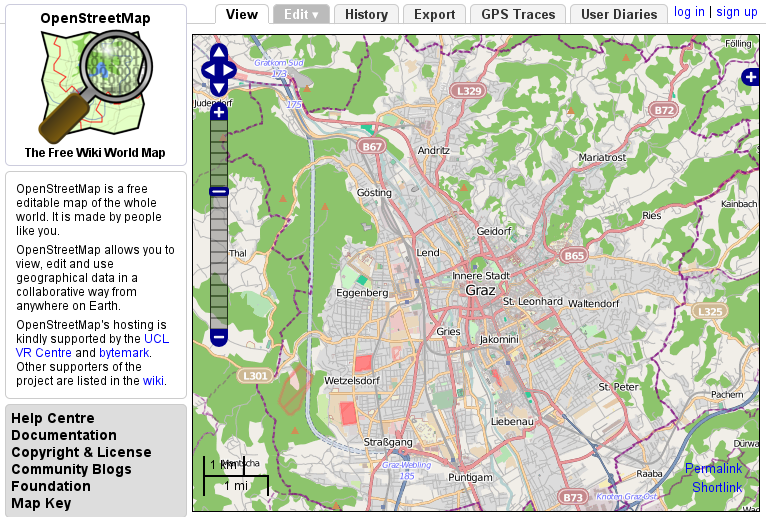
\includegraphics[width=.65\paperwidth]{osm.png}
\end{columns}


\end{frame}

\begin{frame}{Suche}

  \begin{itemize}
    \item vom Speziellen zum Allgemeinen
  \end{itemize}
Bsp.: Bäckerei, Hauptplatz, Graz

\begin{center}
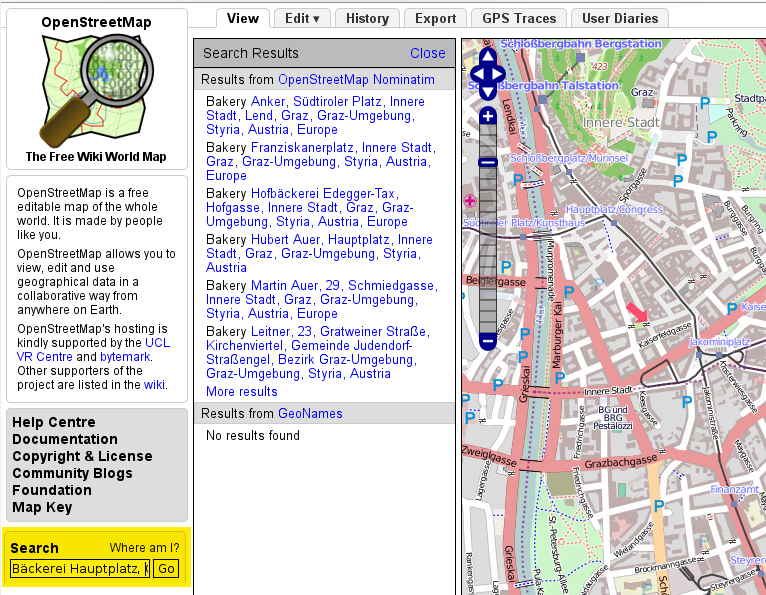
\includegraphics[width=.55\paperwidth]{nominatim.png}
\end{center}

\end{frame}

\begin{frame}{Layerauswahl}
\begin{center}
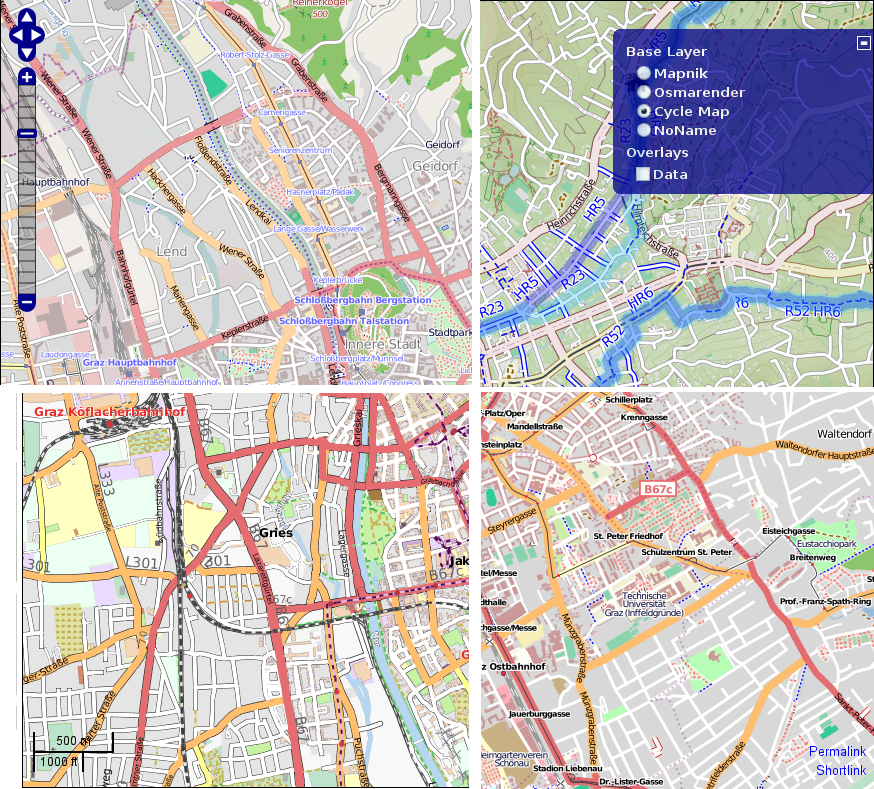
\includegraphics[width=.6\paperwidth]{4layers.png}
\end{center}
\end{frame}


\begin{frame}{Spezialkarten}

  \begin{table}[htbp]
    \centering
    \begin{tabular}{r|l}
      Radkarte  &  \url{http://opencyclemap.org} \\
      Wanderkarte & \url{http://hikebikemap.de} \\
      Rauchfrei-Karte & \url{http://OpenGastroMap.org} \\
      Rollstuhl-Karte & \url{http://wheelmap.org} \\
      Seekarte & \url{http://OpenSeaMap.org} \\
%      Interaktive Informationskarte & http://openstreetbrowser.org
    \end{tabular}
  \end{table}

\end{frame}

\begin{frame}{Radkarte}
\url{http://opencyclemap.org}

\begin{center}
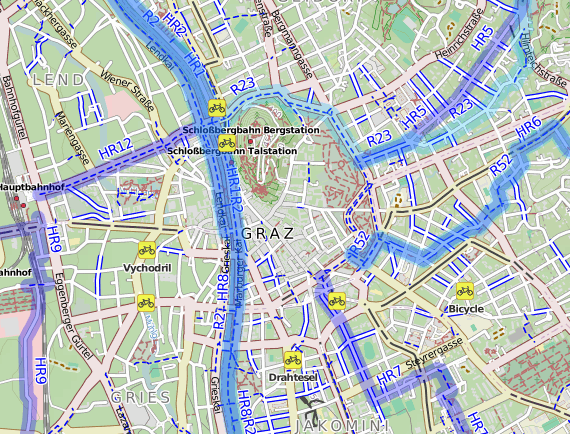
\includegraphics[width=.6\paperwidth]{cyclemap.png}
\end{center}
\end{frame}

\begin{frame}{Wanderkarte}
\url{http://hikebikemap.de}

\begin{center}
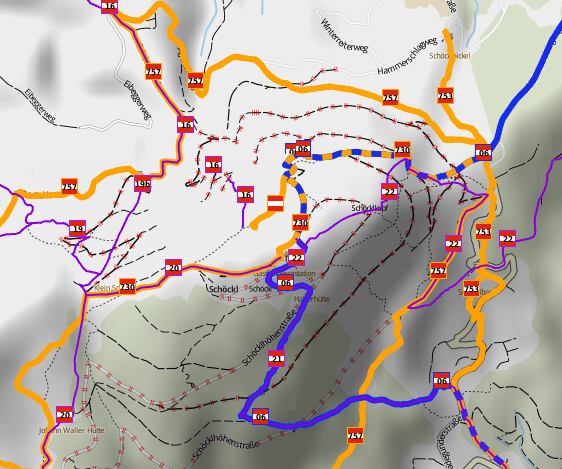
\includegraphics[width=.57\paperwidth]{hike_schoeckl.png}
\end{center}
\end{frame}

\begin{frame}{Rauchfrei-Karte}
\url{http://OpenGastroMap.org}

\begin{center}
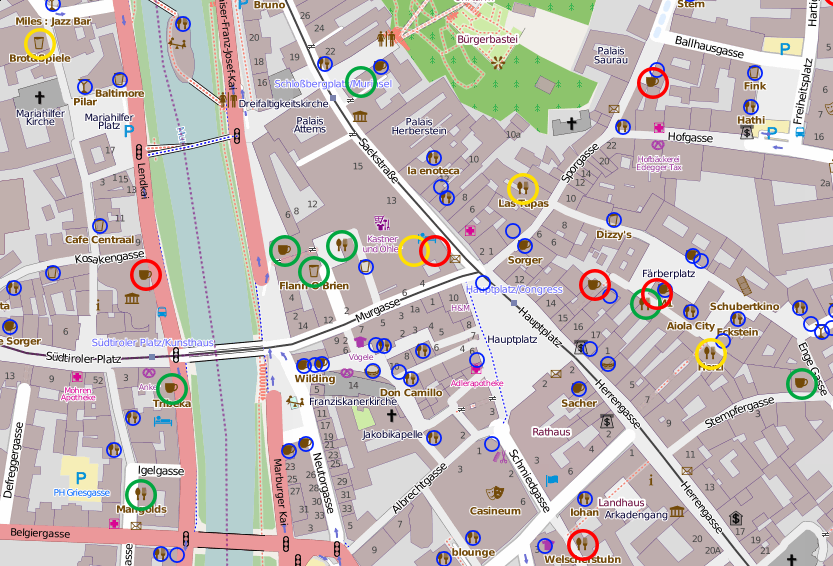
\includegraphics[width=.65\paperwidth]{rauchfrei.png}
\end{center}
\end{frame}

\begin{frame}{Rollstuhl-Karte}
\url{http://wheelmap.org}

\begin{center}
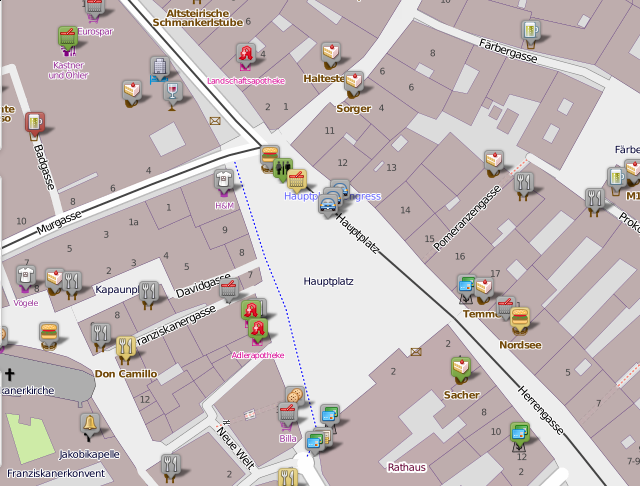
\includegraphics[width=.6\paperwidth]{wheelmap.png}
\end{center}
\end{frame}

\begin{frame}{Seekarte}
\url{http://OpenSeaMap.org}

\begin{center}
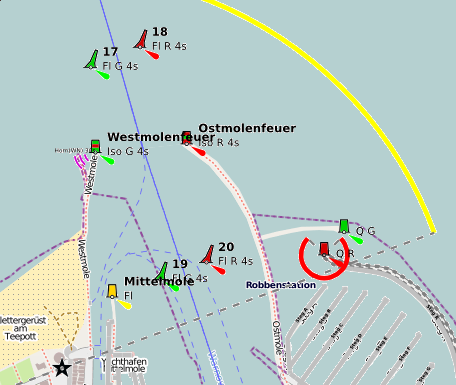
\includegraphics[width=.55\paperwidth]{seamap.png}
\end{center}
\end{frame}


\subsection{Online-Routing}

\begin{frame}{Online-Routing}

Allgemeine Routing-Seiten:\\
Auto, Fußgänger, Fahrrad-Routing

\begin{itemize}
  \item \url{http://openrouteservice.org}
  \item \url{http://maps.cloudmade.com}
\end{itemize}


Spezial-Routing:

\begin{itemize}
  \item Wheelchair-routing: \url{http://rollstuhlrouting.de}
\end{itemize}

\end{frame}


\begin{frame}{OpenRouteService.org}
\url{http://openrouteservice.org}

\begin{center}
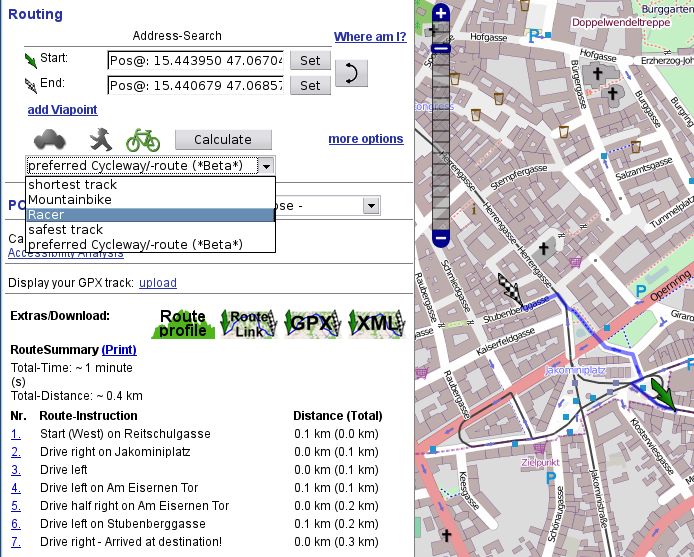
\includegraphics[width=.55\paperwidth]{ors-cycleroute.png}
\end{center}
\end{frame}

%\begin{frame}{CloudMade Maps}
%\url{http://maps.cloudmade.com}

%\begin{center}
%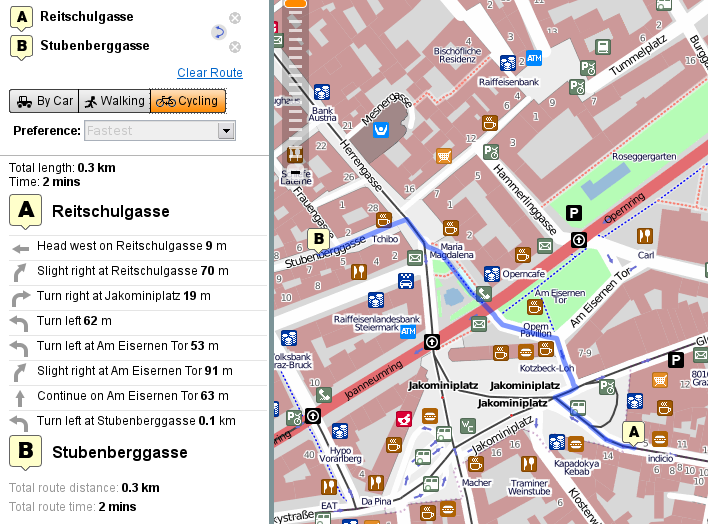
\includegraphics[width=.55\paperwidth]{cloudmade-cycleroute.png}
%\end{center}
%\end{frame}


\subsection{Lizenz}
\begin{frame}{Lizenz}

Derzeit: CC-BY-SA 2.0 
\includegraphics[width=1cm]{cc-by-sa.png} \\
$\Rightarrow$ ``(c) OpenStreetMap contributors, CC-BY-SA''

\begin{itemize}
  \item OpenStreetMap und Lizenztyp müssen genannt werden
  \pause
  \item Tile Usage Policy
\end{itemize}

\pause

Lizenzwechsel zu Open Database License (ODbL)

\begin{itemize}
  \item Probleme mit CC-BY-SA, wenn auf Daten angewendet
  \item Theoritisch müsste jeder einzelne Contributor genannt werden
  \item ODbL löst dieses Problem
\end{itemize}

\pause

Auswirkungen?

Für jeden, der nach dem 12. Mai 2010 bei OSM angefangen hat - keine.

\end{frame}


\subsection{Daten}
\begin{frame}{Daten}

\begin{itemize}
  \item Punkte (Koordinaten), $\Rightarrow$ ``Node'' 
\includegraphics[width=0.5cm]{node.png}
  \item Flächen sind eine Reihe von Nodes, $\Rightarrow$ ``Way'' 
\includegraphics[width=0.5cm]{way.png}
  \item Gruppierungen von Ways $\Rightarrow$ ``Relations'' 
\includegraphics[width=0.5cm]{relation.png}
\end{itemize}

\pause

Jedes Element hat Eigenschaften $\Rightarrow$ ``Tags'', zB:
\begin{itemize}
  \item amenity = Cafe 
\includegraphics[width=0.5cm]{cafe.png}
  \item highway = footway 
\includegraphics[width=1cm]{footway.png}
  \item building = yes  
\includegraphics[width=0.5cm]{building.png}
  \item landuse = farmland 
\end{itemize}

\pause

Was taggen wir?

\pause

Alles :-)

\begin{itemize}
  \item highway=*, landuse=*, shop=*, tourism=*, \dots
  \item ?=*
\end{itemize}

Gebräuchliche Tags und Beschreibungen $\Rightarrow$ Wiki!

\end{frame}

\section{Mitmachen!}

\begin{frame}{Wie kann ich mitmachen?}

\begin{itemize}
  \item Aber da braucht man ein GPS \dots
  \pause
  \item \dots nicht unbedingt!
\end{itemize}

Es gibt viele Möglichkeiten, etwas beizutragen:

\begin{itemize}
  \item Humanitarian OSM Team \href{http://tasks.hotosm.org}{hotosm.org}
  \item Rauchfreie Lokale melden: \href{http://OpenGastroMap.org}{OpenGastroMap}
  \item Rollstuhleignung eintragen: \href{http://wheelmap.org}{wheelmap.org}
  \item Walking Papers
  \item Wissen über deine Umgebung beisteuern
    \begin{itemize}
      \item Bekannte Hausnummern eintragen
      \item Lokale, Geschäfte, \dots
    \end{itemize}
  \item eigene GPS-Tracks zur Verfügung stellen
\end{itemize}

\end{frame}


\begin{frame}{Help}

\begin{itemize}
  \item Erste Station sollte das Wiki sein: \url{wiki.openstreetmap.org}
  \item Immer noch etwas Unklar? $\Rightarrow$ Mailingliste talk-at
  \pause
  \item Stammtisch! In Graz alle 2 Monate - der nächste am Montag im Brot \& Spiele
\end{itemize}

\end{frame}

\section{Danke!}

\begin{frame}{Abschluss}

Folien zum OpenStreetMap-Vortrag für das \href{http://afrikacamp-graz.at}{AfricaCamp 2011} in Graz am 26.11.2011.
\vspace{1cm}

Folien unter 
\includegraphics[width=1cm]{cc-by-sa.png}.
\vspace{1cm}

Erstellt mittels \LaTeX Beamer, source auf Anfrage.
\vspace{1cm}

\href{mailto:michael.maier@student.tugraz.at}{Michael Maier}
\end{frame}

\end{document}
